\chapter{Matériel et méthodes} \label{chap:metho}

Introduction et annonce du plan du chapitre.

\lipsum[1] % génère un paragraphe (à supprimer)


\section{Territoire d’étude} \label{sec:territoire_etude}

\lipsum[1-2] % génère deux paragraphes (à supprimer)


\section{Données} \label{sec:donnees}

\subsection{Données primaires} \label{subsec:donnees_primaires}

\lipsum[1] % génère un paragraphe (à supprimer)


\subsection{Données secondaires} \label{subsec:donnees_secondaires}

\lipsum[1] % génère un paragraphe (à supprimer)


\section{Structuration des données} \label{sec:structuration_donnees}

\lipsum[1] % génère un paragraphe (à supprimer)


\section{Méthodes d’analyse} \label{sec:methodes_analyses}

\subsection{Méthode 1} \label{subsec:methodes1}

\lipsum[1] % génère un paragraphe (à supprimer)


\subsection{Méthode 2} \label{subsec:methodes2}

\lipsum[1] % génère un paragraphe (à supprimer)

\subsubsection{Sous-section} \label{subsubsec:sous_section}

\lipsum[1] % génère un paragraphe (à supprimer)


\subsubsection{Sous-section} \label{subsubsec:sous_section2}

\lipsum[1] % génère un paragraphe (à supprimer)


\subsection{Méthode 3} \label{subsec:methodes3}
Comment numéroter et faire référence à une équation? Les mesures du RMSE et de $R^2$ (équations \ref{eq:rmse} et \ref{eq:r2}) sont utilisées...


\begin{equation}
\text{RMSE} = \sqrt{\frac{\sum_{i=1}^{n}\left(y_i - \hat{y}_i\right)^2}{n}} 
\label{eq:rmse}
\end{equation}

\begin{equation}
R^2 = \frac{\sum_{i=1}^{n}\left(\hat{y}_i - \bar{y}\right)^2}{\sum_{i=1}^{n}\left(y_i - \bar{y}\right)^2} 
\label{eq:r2}
\end{equation}

L'équation de la régression linéaire multiple s'écrit :

\begin{equation}
Y = X\beta + \epsilon \quad \text{avec :}
\label{eq:regression_lineaire}
\end{equation}
\begin{itemize}
    \item $Y$ est un vecteur de dimension $n \times 1$ pour la variable dépendante, soit une colonne avec $n$ observations.
    \item $X$ est une matrice de dimension $n \times (k+1)$ pour les $k$ variables indépendantes, incluant une autre colonne pour la constante.
    \item $\beta$ est un vecteur de dimension $k+1$, soit les coefficients de régression pour les $k$ variables et la constante.
    \item $\epsilon$ est un vecteur de dimension $n \times 1$ pour les résidus.
\end{itemize} 

L'analyse des résultats du modèle est présentée dans le tableau \ref{tab:tableau1}.

\begin{table}[H]
    \centering % tableau centré sur la largeur de la page
    \singlespacing % interligne simple
    \begin{threeparttable}
    \caption{Premier tableau du chapitre 3}
    \label{tab:tableau1}
    \renewcommand{\arraystretch}{1.2}
    \begin{tabular}{l c c c}
    \hline % Ligne
    \textbf{Colonne A} & \textbf{Colonne B} & \textbf{Colonne C} & \textbf{Colonne D} \\
    \hline % Ligne
    Texte & Texte & Texte & Texte \\
    Texte & Texte & Texte & Texte \\
    Texte & Texte & Texte & Texte \\
    Texte & Texte & Texte & Texte \\
    Texte & Texte & Texte & Texte \\
    \hline % Ligne
    \end{tabular}
    \begin{tablenotes}[flushleft]
    \small
    \item \textit{Note :} facultatif.
    \end{tablenotes}
    \end{threeparttable}
\end{table}

Différentes fonctions Kernel peuvent être utlisées (figure~\ref{fig:kernels}).

\begin{figure}[H]
    \centering
    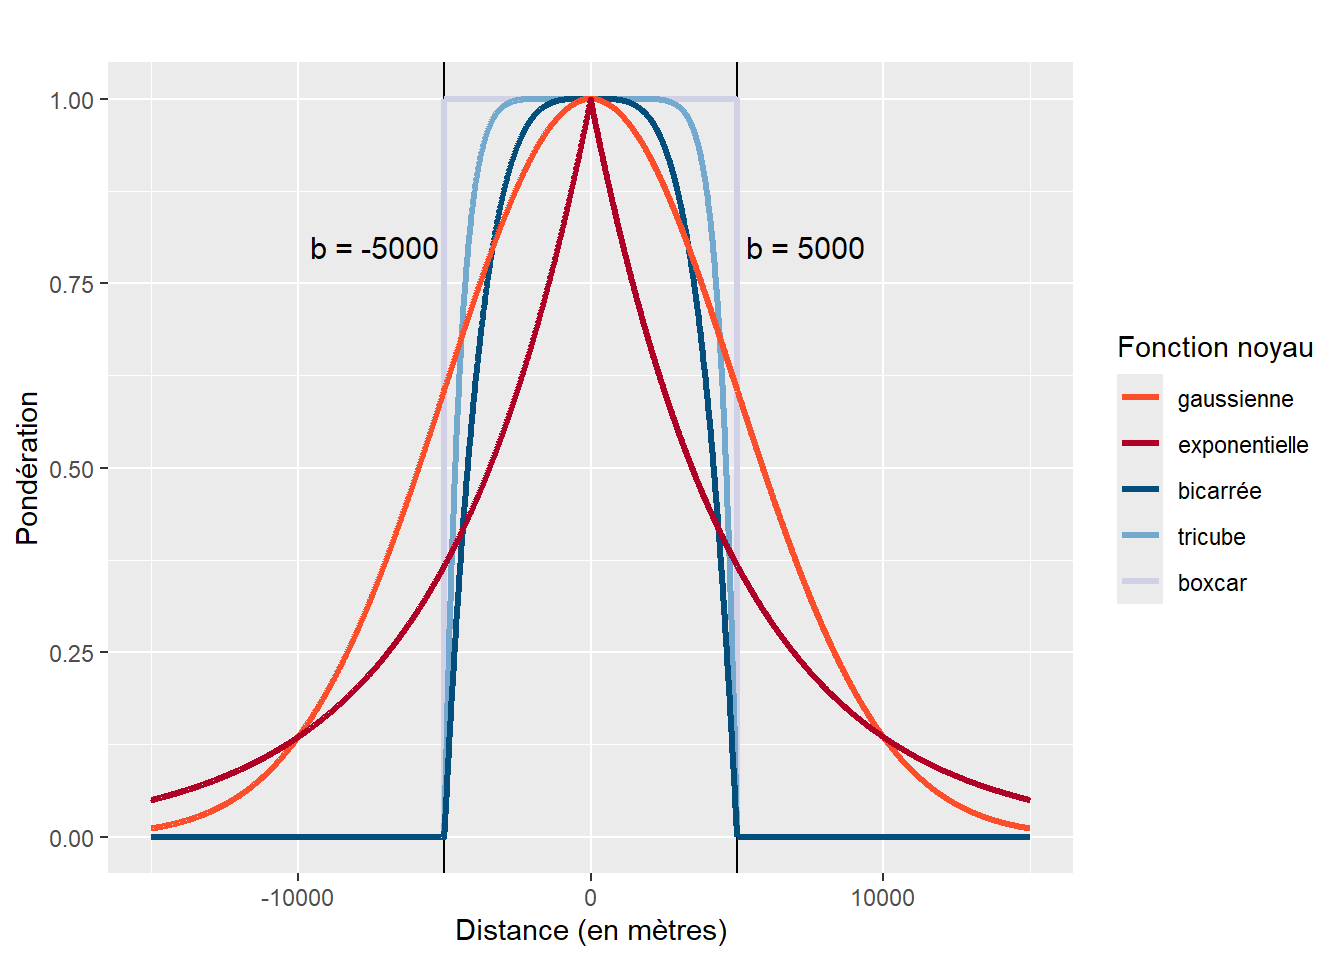
\includegraphics[width=0.8\textwidth]{figures/kernels.png}
    \caption{Fonctions noyaux (kernel) pour définir la matrice de pondération W(i)}
    \label{fig:kernels}
\end{figure}

\begin{table}[H]
    \centering % tableau centré sur la largeur de la page
    \singlespacing % interligne simple
    \begin{threeparttable}
    \caption{Deuxième tableau du chapitre 3}
    \label{tab:tableau2}
    \renewcommand{\arraystretch}{1.2}
    \begin{tabular}{l c c c}
    \hline % Ligne
    \textbf{Colonne A} & \textbf{Colonne B} & \textbf{Colonne C} & \textbf{Colonne D} \\
    \hline % Ligne
    Texte & Texte & Texte & Texte \\
    Texte & Texte & Texte & Texte \\
    Texte & Texte & Texte & Texte \\
    Texte & Texte & Texte & Texte \\
    Texte & Texte & Texte & Texte \\
    \hline % Ligne
    \end{tabular}
    \begin{tablenotes}[flushleft]
    \small
    \item \textit{Note :} facultatif.
    \end{tablenotes}
    \end{threeparttable}
\end{table}

\newpage

En théorie des graphes, l'algorithme de Dijkstra résout le problème du plus court chemin
(algorithme~\ref{algo:dijkstra}).


\begin{algorithm}[H]
\DontPrintSemicolon
\KwIn{Un graphe $G = (V, E)$ avec des poids $w(u,v) \geq 0$ et un sommet source $s \in V$}
\KwOut{Les distances minimales $d[v]$ de $s$ à chaque sommet $v \in V$, et les prédécesseurs}
\BlankLine
\ForEach{$v \in V$}{
    $d[v] \leftarrow \infty$ \;
    $\textit{prec}[v] \leftarrow$ indéfini \;
}
$d[s] \leftarrow 0$ \;
$Q \leftarrow V$ \tcp*{file de priorité contenant tous les sommets}
\While{$Q \neq \emptyset$}{
    $u \leftarrow$ sommet dans $Q$ avec la plus petite valeur $d[u]$ \;
    Supprimer $u$ de $Q$ \;
    \ForEach{$v$ voisin de $u$}{
        \If{$v \in Q$ \textbf{et} $d[u] + w(u,v) < d[v]$}{
            $d[v] \leftarrow d[u] + w(u,v)$ \;
            $\textit{prec}[v] \leftarrow u$ \;
        }
    }
}
\Return{$d$ et $\textit{prec}$} \;
\caption{Algorithme de Dijkstra}
\label{algo:dijkstra}
\end{algorithm}

Pour intégrer des acronymes dans le texte, utiliser la commande \textbf{\string\gls\{nom-acronyme\}}. Les acronymes doivent être préalablement définis dans le fichier \textbf{auxilaires/acronymes.tex}. Un hyperlien sur l'acronomyme renvoie ainsi automatiquement à la liste des acronymes.

Voici un exemple, les principaux indices de végétation sont\,: 

\begin{itemize}
    \item \gls{ndvi}
    \item \gls{rvi}
    \item \gls{savi}
    \item \gls{osavi}
    \item \gls{msavi}
    \item \gls{ndre}
    \item \gls{ndwi}
    \item \gls{msi}
\end{itemize}

Note : La commande \textbf{\string\gls\{nom-acronyme\}} gérera automatiquement l'affichage du nom complet (Indice de végétation par différence normalisée) lors de sa première occurrence, puis de son acronyme seul par la suite.

Le plus couramment utilisé et connu est le \gls{ndvi}

Avec les \gls{sig}.

Selon l'\gls{onu} et l'\gls{oms}.
